\chapter{System Design}
\section{System Overview}
FinSight is an AI-powered financial analytics and recommendation platform designed for investors and analysts. It integrates natural language understanding, time-series forecasting, vector search, and \acf{RAG} to provide end-to-end financial insights. The system design is shown in Figure 4.1.
\begin{figure}[ht!] % supposedly places it here ...
	\centering
	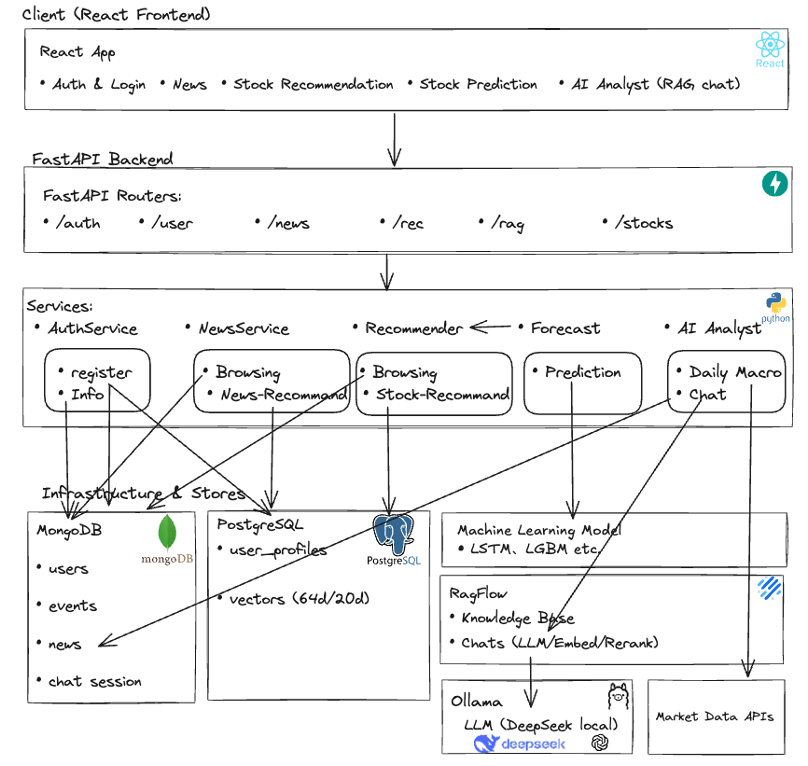
\includegraphics[width=1\linewidth]{images/system_design.png}
	\caption[system design]{Finsight system design}
	\label{fig:system_design}
\end{figure}

\subsection{System Architecture}

\begin{longtable}{p{3cm}p{10cm}}
\toprule
\textbf{Module} & \textbf{Description} \\
\midrule
News Module & Fetches financial news via Google \acs{RSS} and APIs, performs \acs{NLP} parsing and vectorization. \\
Recommendation Module & Combines user profile embeddings and stocks vectors for personalized ranking. \\
Forecast Module & Predicts stock prices using \acs{ARIMA}, Prophet, \acs{LGBM}, \acs{LSTM}, and ensemble models. \\
RAG Module & Integrates RagFlow for retrieval-augmented question answering. \\
User Profile Module & Maintains user semantic (64D) and preference (20D) embeddings and stores users base information. \\
Auth \& User Service & Handles registration, login, JWT authentication, and profile setup. \\
Database Client & Manages MongoDB, PostgreSQL, and SSH tunneling. \\
\bottomrule
\end{longtable}

\subsection{Data Flow and Integration}
\begin{enumerate}[leftmargin=1.5em]
    \item Users register for this platform. Each user will get his own user profile(a 20D vector that representsing their investment interests). Based on users' behavior(like click \ like \ dislike) to adjust their profile vector.
    \item The frontend sends a REST API request to FastAPI endpoints such as \texttt{/forecast}, \texttt{/stocks},\texttt{/news}, or \texttt{/rag}.
    \item The backend loads user profiles, news data, stock data, or knowledge base content.
    \item Depending on the task, it calls news modules, forecasting models, RAG reasoning, or recommendation logic.
    \item The backend returns structured JSON results visualized by the frontend dashboard.
\end{enumerate}

\subsection{Tech Stack}

\begin{longtable}{p{3cm}p{11cm}}
\toprule
\textbf{Layer} & \textbf{Technology and Description} \\
\midrule
Frontend & React + Vite + TailwindCSS + Recharts for interactive dashboards. \\
Backend & FastAPI (Python 3.12+) with modular routers and service layers. \\
Database & MongoDB for document data; PostgreSQL + pgvector for vector storage. \\
Machine Learning & Prophet, ARIMA, LightGBM, LSTM, Transformer and Seq2Seq forecasting. \\
LLM / RAG & RagFlow for retrieval-augmented reasoning; DeepSeek-8B and OpenAI embeddings; Ollama for llm services. \\
Infrastructure & Docker, Uvicorn, SSH tunnel, NUS \acs{HPC}, and AWS EC2 deployment. \\
\bottomrule
\end{longtable}

% \section{User Register Module}



\section{News Browsing Module}

Design goals were: a clean feed, de-duplication across sources, light personalization, and a smooth API surface. In practice we ship a two-vector design (semantic 64-d, preference 20-d), an \textbf{exclude-seen} filter backed by Mongo events, and a \textbf{dual refresh mode} that keeps first-paint fast while allowing small, quota-friendly real-time pulls. The front end renders a \(3\times 3\) grid with cached paging (previous/next/jump), so user actions immediately influence subsequent pages without blocking the UI.

\subsection{Overall Architecture Design}
The module follows a clear \textbf{Service ⟂ Repository} split with thin HTTP endpoints:

\begin{itemize}
  \item \textbf{Datastores.} News and events are stored in \textbf{MongoDB} (documents: title, url, source, \texttt{published\_at}, tickers, sector, topics, sentiment, plus 20-d profile vector \(\mathbf{p}_a\)); \textbf{PostgreSQL + pgvector} holds the normalized 64-d semantic embeddings for articles and the 20-d user profile \(\mathbf{u}\in\mathbb{R}^{20}\).
  \item \textbf{Service core (NewsService).} Orchestrates candidate gathering, scoring, and post-filters. It also coordinates a tiny ``trickle'' ingestion when \texttt{refresh=1}---pulling \(\le 3\) fresh items using symbol hints, upserting them, then re-ranking together with the local corpus.
  \item \textbf{Repositories.}
    \begin{itemize}
        \item \texttt{NewsRepo} (Mongo) for latest/news lookup and upserts.
        \item \texttt{PgProfileRepo} (Postgres) for \(\mathbf{u}\) updates and vector math.
        \item \texttt{EventRepo} (Mongo) logging \texttt{click/like/bookmark}, plus a compact \textbf{toggle} collection for idempotent ``add'' and reversible ``remove''.
    \end{itemize}
  \item \textbf{HTTP surface (FastAPI).}
    \begin{itemize}
        \item \texttt{GET /rec/user/news} -- ranked results with \texttt{refresh=\{0,1\}}, \texttt{symbols=}, \texttt{exclude\_hours=} (exclude seen).
        \item \texttt{POST /users/event/\{click|like|bookmark\}} -- log behavior and update \(\mathbf{u}\).
        \item \texttt{GET /debug/news/latest} -- fast first-paint sample (9 items) directly from the DB.
    \end{itemize}
\end{itemize}

This layout keeps hot read paths short (DB-only) while still supporting tiny real-time updates, and isolates vector math and schema evolution behind stable service methods.

\subsection{Candidates, Scoring, and Ranking}

At request time, the service constructs a candidate set and ranks it with a compact, interpretable score. If \texttt{refresh=0}, candidates are simply the latest \(K\) items from Mongo; if \texttt{refresh=1}, the service first pulls a \textbf{very small} batch of fresh articles (guided by \textbf{top-3 tickers} on the current page), upserts, and then re-queries latest. After candidate assembly we apply \textbf{exclude-seen} using recent user events (click/like/bookmark) within a sliding window (e.g., 30 days), then de-dup strictly by \texttt{news\_id}.

The final score blends preference match, recency, and page-level diversity, then clips to \([0,1]\):
\[
\mathrm{score}(u,a)\;=\;
\alpha\,\cos\!\big(\mathbf{u},\mathbf{p}_a\big)
\;+\;\beta\,f_{\text{recency}}(a)
\;+\;\gamma\,f_{\text{diversity}}(a\mid\mathcal{S})
\;\;\in[0,1].
\]
Here \(\mathbf{p}_a\in\mathbb{R}^{20}\) is the article’s 20-d preference vector aligned with our sector/bucket basis; \(f_{\text{recency}}\) mildly favors newer items; \(f_{\text{diversity}}\) discourages near-duplicates within the top-\(N\) slate \(\mathcal{S}\). We then take the top \(N=9\) for one page and return \(\{\text{title, url, source, published\_at, tickers, sector}\}\) for rendering.

\subsection{Feedback Loop and Online Profile Updates}

Interactions close the loop via \textbf{append-only events} in Mongo and immediate updates to the 20-d user profile \(\mathbf{u}\) in Postgres. Each click carries a weight:
\[
w \;=\; 1 \;+\; 0.5\,\mathbf{1}[\text{dwell}\ge 10\text{s}]
\;+\; 0.5\,\mathbf{1}[\texttt{liked}]
\;+\; 0.5\,\mathbf{1}[\texttt{bookmarked}].
\]
For \textbf{positive} actions (add) we nudge toward the article’s preferences:
\[
\mathbf{u} \;\leftarrow\; \mathbf{u} \;+\; \eta\,w\,\mathbf{p}_a.
\]
For \textbf{removals} (e.g., un-like / un-bookmark) we apply a \textbf{fixed decrement} to the same dimensions---simple, stable, and snapshot-free:
\[
\mathbf{u} \;\leftarrow\; \mathbf{u} \;-\; \eta_r\,\mathbf{p}_a,
\qquad \eta_r \ll \eta .
\]
We de-duplicate ``add'' by a \((\texttt{user}, \texttt{news}, \texttt{type})\) toggle so repeated likes do not double-count, and we no-op ``remove'' if the toggle is already off. In practice this yielded \textbf{monotone} improvements after positive feedback and sensible reversion after removals, without the fragility of storing/restoring full vector snapshots.

\subsection{Latency, Caching, and Refresh Modes}

To keep the interface responsive and protect API quotas, we maintain two coordinated modes:

\begin{itemize}
  \item \textbf{DB-only paging (\texttt{refresh=0}).} Used for initial paint and most page turns. The front end caches pages locally (arrays of 9 items) and keeps a set of \texttt{seenIds}. ``Previous'' and page jumps are pure client operations; ``Next'' is also cached unless the user is already on the \textbf{last} page.
  \item \textbf{Trickle refresh (\texttt{refresh=1}).} Triggered only when the user is on the last page and presses ``Next.'' The service pulls at most a few \textbf{fresh articles} (guided by the current page’s top-3 tickers), upserts, and re-ranks together with the corpus---delivering freshness at a \textbf{tiny} marginal cost.
\end{itemize}

In both modes, the server still enforces exclude-seen and de-dup, ensuring the \(3\times 3\) slate remains \textbf{novel}. The front end never blocks on re-ranking to show cached pages; it only waits on network when specifically expanding the tail with \texttt{refresh=1}.

\section{Stock Recommendation Module Architecture}

\subsection{Overall Architecture Design}

The stock recommendation module employs a sophisticated \textbf{microservices} architecture that seamlessly integrates with the broader investment platform. As illustrated in Figure \ref{fig:recommend_overview}, the module operates as a central intelligence hub, processing user preferences, market data, and financial metrics to generate personalized investment recommendations.

\begin{figure}[ht!] % supposedly places it here ...
	\centering
	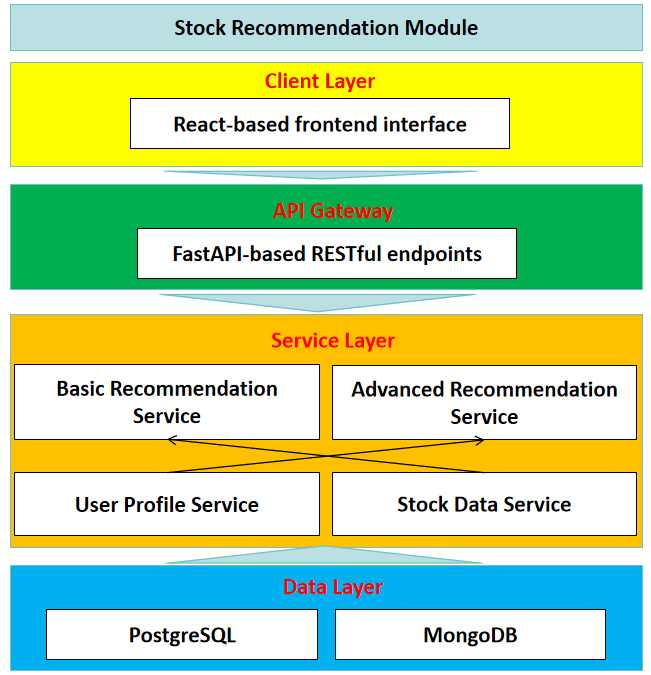
\includegraphics[scale=0.8]{images/stock_recommend/recommend_overview.png}
	\caption{Stock Recommendation System Architecture}
	\label{fig:recommend_overview}
\end{figure}


The architecture is designed for scalability and real-time performance, employing asynchronous processing patterns and intelligent caching strategies. The module supports multiple recommendation strategies that can be dynamically selected based on user preferences and market conditions.

\subsection{Basic Recommendation Engine}

The basic recommendation engine forms the \textbf{foundation} of our stock recommendation system, implementing a sophisticated vector similarity approach combined with intelligent diversification.

\textbf{Vector Similarity Foundation:}
The core algorithm computes \textbf{cosine} similarity between 20-dimensional user and stock vectors:

\begin{equation}
\text{Similarity}(\mathbf{U}, \mathbf{S}) = \frac{\sum_{i=1}^{20} U_i \cdot S_i}{\sqrt{\sum_{i=1}^{20} U_i^2} \cdot \sqrt{\sum_{i=1}^{20} S_i^2}}
\end{equation}

Where $\mathbf{U}$ represents the user's 20-dimensional preference vector and $\mathbf{S}$ represents the stock's 20-dimensional characteristic vector. The 20 dimensions are carefully engineered to capture both sector preferences (dimensions 0-10) and investment style preferences (dimensions 11-19).

\textbf{Diversification Enhancement:}
To prevent over-concentration in specific sectors, the system implements a dynamic diversification mechanism:

\begin{equation}
\text{Final Score} = \text{Raw Similarity} - \alpha \cdot \mathbb{I}_{\text{sector seen}}
\end{equation}

Where $\alpha$ is the diversity factor (configurable from 0 to 0.3) and $\mathbb{I}_{\text{sector seen}}$ is an indicator function that equals 1 if the sector has already been selected in the current recommendation batch. This approach ensures that even if multiple technology stocks have high similarity scores, the system will prioritize including stocks from underrepresented sectors.

This approach ensures that recommendations are both personalized to user preferences and strategically diversified across market sectors.

\subsection{Advanced Multi-Objective Recommendation Engine}

The advanced recommendation engine represents a significant evolution beyond basic similarity matching, implementing a sophisticated multi-objective optimization framework that balances four critical investment dimensions.

\textbf{Multi-Objective Optimization Framework:}
The final recommendation score is computed as a weighted combination of four component scores:

\begin{equation}
\text{Final Score} = w_p \cdot S_p + w_r \cdot S_r + w_d \cdot S_d + w_t \cdot S_t
\end{equation}

Each component score represents a distinct investment objective:

\textbf{Preference Similarity Score ($S_p$)}:
This component measures alignment between user preferences and stock characteristics using the same 20-dimensional vector similarity as the basic engine, but with additional normalization to ensure compatibility with other components.

\textbf{Risk-Adjusted Return Score ($S_r$)}:
This sophisticated component evaluates the risk-reward profile of each stock:

\begin{equation}
S_r = \frac{\text{Expected Return}}{\max(\text{Volatility}, 0.01)}
\end{equation}

Expected return is estimated using a multi-factor model:
\begin{equation}
\text{Expected Return} = 0.3 \cdot R_{\text{historical}} + 0.4 \cdot R_{\text{growth}} + 0.3 \cdot R_{\text{valuation}}
\end{equation}

Where:
\begin{itemize}
\item $R_{\text{historical}}$: 3-month price momentum normalized to annual returns
\item $R_{\text{growth}}$: Revenue growth projections from fundamental analysis
\item $R_{\text{valuation}}$: Valuation reversal effect based on P/E ratios
\end{itemize}

Volatility is computed from 30-day historical price movements and annualized for consistency.

\textbf{Diversification Benefit Score ($S_d$)}:
This component evaluates each stock's contribution to portfolio diversification:

\begin{equation}
S_d = 1 - \text{Sector Concentration}
\end{equation}

Sector concentration is calculated as:
\begin{equation}
\text{Sector Concentration} = \frac{\text{Number of stocks in sector}}{\text{Total stocks in universe}}
\end{equation}

This ensures that stocks from underrepresented sectors receive higher diversification scores, promoting balanced portfolio construction.

\textbf{Market Timing Score ($S_t$)}:
This dynamic component adapts recommendations to current market conditions:

\begin{equation}
S_t = \begin{cases}
\beta \cdot 0.8 + \text{Dividend Yield} \cdot 5 \cdot 0.2 & \text{if bear market} \\
\beta \cdot 0.8 + \text{Growth Score} \cdot 0.2 & \text{if bull market} \\
(1 - \text{Volatility}) \cdot 0.5 + \text{Valuation Score} \cdot 0.5 & \text{if sideways market}
\end{cases}
\end{equation}

Market regime detection analyzes SPY ETF data using 3-month returns and volatility:
\begin{itemize}
\item \textbf{Bull Market}: Return > 10\% and Volatility < 20\%
\item \textbf{Bear Market}: Return < -5\% and Volatility > 25\%
\item \textbf{Sideways Market}: All other conditions
\end{itemize}

\textbf{Dynamic Weight Adjustment:}
The system employs risk-profile-based weight configurations:

\begin{table}[h]
\centering
\caption{Multi-Objective Weight Configuration by Risk Profile}
\begin{tabular}{|l|c|c|c|c|}
\hline
\textbf{Risk Profile} & \textbf{Preference ($w_p$)} & \textbf{Risk Return ($w_r$)} & \textbf{Diversification ($w_d$)} & \textbf{Timing ($w_t$)} \\
\hline
Conservative & 0.2 & 0.4 & 0.3 & 0.1 \\
Balanced & 0.3 & 0.4 & 0.2 & 0.1 \\
Aggressive & 0.3 & 0.5 & 0.1 & 0.1 \\
\hline
\end{tabular}
\end{table}

\subsection{Real-time User Behavior Integration}

Both recommendation engines incorporate real-time user feedback to continuously refine preference models:

\begin{equation}
\mathbf{U}_{t+1} = \mathbf{U}_t + \eta \cdot (\mathbf{S} - \mathbf{U}_t)
\end{equation}

Where $\eta$ is the learning rate that varies by behavior type:
\begin{itemize}
\item $\eta = 0.05$ for click interactions
\item $\eta = 0.20$ for favorite/dislike actions
\item $\eta = -0.20$ for removal of previous interactions
\end{itemize}

This adaptive learning mechanism ensures that the system evolves with user preferences, providing increasingly relevant recommendations over time.




% ==========================================================================================
\section{Stock Trend Prediction Module}

The Stock Forecasting module forms one of the core intelligent reasoning components of the FinSight system. 
It provides users with \textbf{real-time price forecasting} capabilities powered by machine learning and time-series models.
The system integrates a FastAPI-based backend with a React-based frontend, enabling seamless interaction and visualization.

\subsection{System Architecture}

The stock prediction module forms a core component of the FinSight system, providing short-horizon predictions such as one-day, seven-day, and thirty-day forward prices.  
We demonstrate familiarity with \textbf{\acf{MLOps}} here. It adopts a microservice architecture that \textbf{separates responsibilities} between data processing, model inference, and user presentation.  
The backend, implemented in Python using the FastAPI framework, exposes several endpoints.
These endpoints handle data retrieval, model orchestration, and forecast generation.  
Historical price data are stored in MongoDB database, where each document contains time-series data represented as a list of date-close pairs.  
The forecasting service reads this data, invokes the appropriate prediction models, and returns structured results through a REST interface.

On the frontend,  
The user can select a stock ticker from the recommandation tickers' list, and the interface presents both the last seven actual closing prices and the predicted trend for upcoming horizons.  
This integration enables a smooth interaction between data analytics and visualization, delivering both reasoning and interpretability to end users.

The \textbf{Stock Trend Prediction Module Design} is shown in Figure 4.3

\begin{figure}[ht!] 
	\centering
	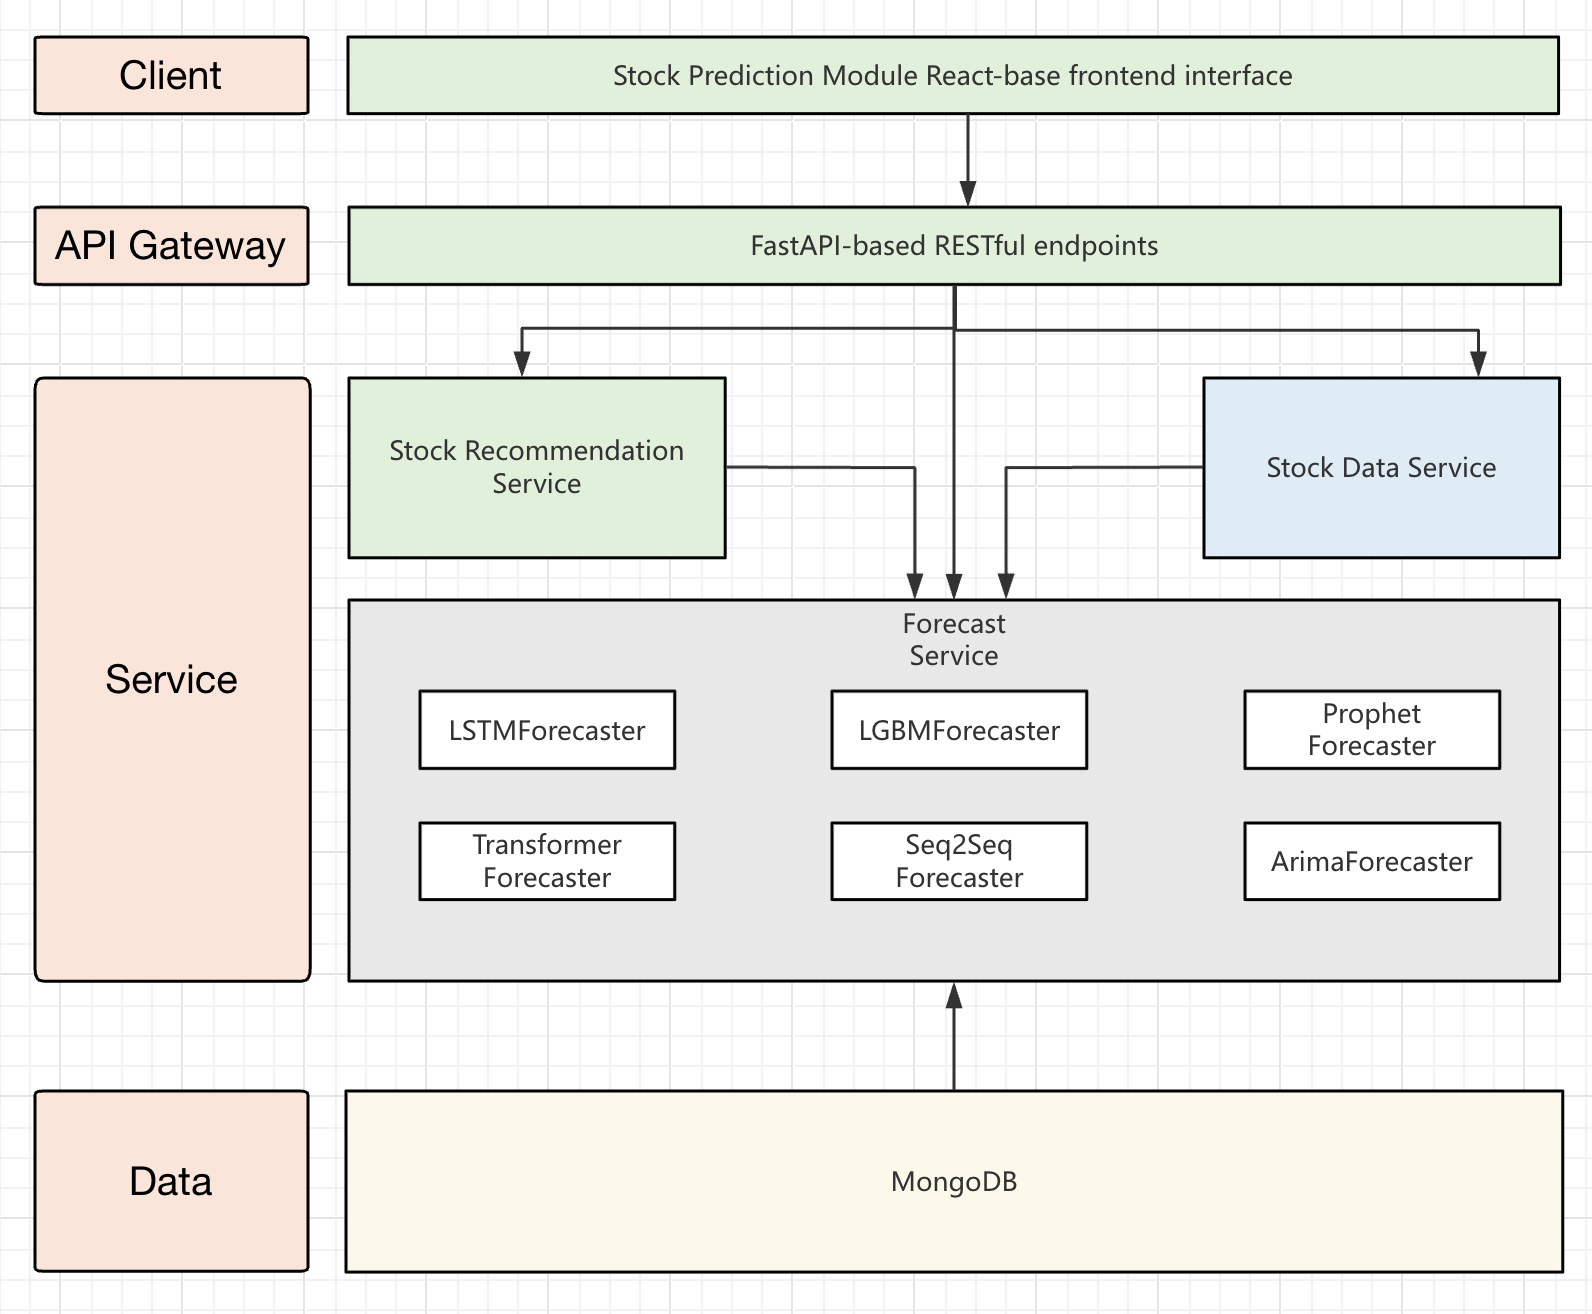
\includegraphics[width=1\linewidth]{images/prediction/arch.png}
	\caption[system design]{Stock Trend Prediction Module Design}
\end{figure}


\subsection{Frontend and Backend Data Processing}

The data flow between the frontend and backend follows a clear \textbf{five-stage} pipeline.  
\textbf{First}, the user selects a ticker symbol within the interface.  
The \textbf{frontend then} issues two asynchronous requests to retrieve the most recent seven actual closing prices.  
Upon receiving these requests, the \textbf{backend} loads the corresponding historical series from our MongoDB database, performs validation, and automatically determines which forecasting model or ensemble to use based on data length and volatility.  
The \textbf{chosen model} then produces a list of predicted values, each associated with a forecast horizon in days and optionally a confidence score.  
All results are \textbf{normalized} into a unified \texttt{ForecastResult} structure, which contains the ticker symbol, current price, model name, and an array of prediction points.

On the frontend side, the two responses are merged into a continuous timeline that combines historical and future values.  
Dates for predicted points are generated by adding the forecast horizon to the current date, ensuring chronological alignment.  
The React component then renders a dual-line chart using the Recharts library, where the solid line represents actual historical prices and the dashed line displays the predicted trajectory.  
When available, confidence intervals can also be visualized as shaded bands around the prediction curve. 

Through this bidirectional communication pipeline, users experience a real-time, interpretable forecasting workflow that blends reasoning and visualization.

\subsection{Forecaster Types and Selection}

The forecasting service integrates a diverse set of models organized into three methodological families. 

The forecasting engine integrates multiple models spanning statistical, machine learning, and deep learning approaches.  
Each model family contributes a distinct reasoning capability to handle different market conditions and data characteristics.  
A summary of these forecasters is given below:

\begin{itemize}

  \item \textbf{LSTM (Long Short-Term Memory).}
  
  LSTM is a \textbf{recurrent neural network} architecture capable of learning long-range temporal dependencies.
  It aims at mitigating the vanishing gradient problem commonly encountered by traditional RNNs.
  It excels in capturing nonlinear price dynamics and is particularly effective with large, continuous datasets.

  An LSTM unit consists of \textbf{a cell and three gates}---input, forget, and output---that regulate the flow of information.
The cell preserves information across time, while the gates determine what to discard, store, or output based on the current input and previous state.
This selective control enables the network to retain long-term dependencies and make accurate sequential predictions.

The compact form of the equations for the forward pass of an LSTM cell with a forget gate is given by:

\begin{align}
f_t &= \sigma_g(W_f x_t + U_f h_{t-1} + b_f), \\
i_t &= \sigma_g(W_i x_t + U_i h_{t-1} + b_i), \\
o_t &= \sigma_g(W_o x_t + U_o h_{t-1} + b_o), \\
\tilde{c}_t &= \sigma_c(W_c x_t + U_c h_{t-1} + b_c), \\
c_t &= f_t \odot c_{t-1} + i_t \odot \tilde{c}_t, \\
h_t &= o_t \odot \sigma_h(c_t),
\end{align}

where the initial values are \( c_0 = 0 \) and \( h_0 = 0 \), and the operator \( \odot \) denotes the element-wise product.  
The subscript \( t \) indexes the time step.

\paragraph{\textbf{Variables}}
Let superscripts \( d \) and \( h \) refer to the number of input features and hidden units, respectively:
\begin{itemize}
    \item \( x_t \in \mathbb{R}^{d} \): input vector to the LSTM unit,
    \item \( f_t \in (0,1)^{h} \): forget gate's activation vector,
    \item \( i_t \in (0,1)^{h} \): input/update gate's activation vector,
    \item \( o_t \in (0,1)^{h} \): output gate's activation vector,
    \item \( \tilde{c}_t \in (-1,1)^{h} \): cell input activation vector,
    \item \( c_t \in \mathbb{R}^{h} \): cell state vector,
    \item \( h_t \in (-1,1)^{h} \): hidden state vector (also known as the output vector),
    \item \( W \in \mathbb{R}^{h \times d}, \; U \in \mathbb{R}^{h \times h}, \; b \in \mathbb{R}^{h} \): weight matrices and bias vectors learned during training.
\end{itemize}

\paragraph{Activation \textbf{Functions}}
\begin{itemize}
    \item \( \sigma_g \): sigmoid activation function,
    \item \( \sigma_c \): hyperbolic tangent function,
    \item \( \sigma_h \): hyperbolic tangent function, or the identity function \( \sigma_h(x) = x \) in the peephole LSTM variant.
\end{itemize}


  \item \textbf{ARIMA (Auto-Regressive Integrated Moving Average).}  
  
  A classical time-series model that captures \textbf{autocorrelation patterns and local trends}.  
  It performs well for stationary or mildly non-stationary data and is computationally efficient for short horizons.
  We use non-seasonal ARIMA model in the Finsight prediction module.

\textbf{Non-seasonal} ARIMA models are usually denoted as \( \mathrm{ARIMA}(p, d, q) \), 
where the parameters \( p, d, q \) are non-negative integers.  
Here, \( p \) is the order (number of time lags) of the \textit{autoregressive} part of the model,  
\( d \) is the degree of differencing (the number of times the data have had past values subtracted),  
and \( q \) is the order of the \textit{moving-average} part.  


Given time series data \( X_t \), where \( t \) is an integer index and \( X_t \) are real numbers,  
an \( \mathrm{ARMA}(p', q) \) model is given by

\begin{equation}
X_t - \alpha_1 X_{t-1} - \cdots - \alpha_{p'} X_{t-p'} 
= \varepsilon_t + \theta_1 \varepsilon_{t-1} + \cdots + \theta_q \varepsilon_{t-q},
\end{equation}

or equivalently,

\begin{equation}
\left( 1 - \sum_{i=1}^{p'} \alpha_i L^i \right) X_t
= \left( 1 + \sum_{i=1}^{q} \theta_i L^i \right) \varepsilon_t,
\end{equation}

where \( L \) is the \textit{lag operator}, 
the \( \alpha_i \) are the parameters of the autoregressive part of the model, 
the \( \theta_i \) are the parameters of the moving average part, 
and the \( \varepsilon_t \) are the error terms.  
The error terms \( \varepsilon_t \) are generally assumed to be 
independent and identically distributed (i.i.d.) random variables 
sampled from a normal distribution with zero mean.


  \item \textbf{Transformer.}

  The Transformer forecaster adopts a \textbf{self-attention}-based architecture that replaces recurrent computation 
with parallelizable attention mechanisms.  
Unlike RNNs, which process sequences step by step, 
Transformers model all time-step relationships simultaneously, 
allowing them to learn long-range dependencies and contextual interactions more efficiently.

Given an input matrix \( X \in \mathbb{R}^{L \times d} \) of historical embeddings, 
the self-attention mechanism computes:
\begin{equation}
\mathrm{Attention}(Q, K, V) = \mathrm{softmax}\!\left(\frac{QK^{\top}}{\sqrt{d_k}}\right)V,
\end{equation}
where \( Q = XW_Q \), \( K = XW_K \), and \( V = XW_V \) 
are the query, key, and value projections with learnable matrices \( W_Q, W_K, W_V \in \mathbb{R}^{d \times d_k} \).  
This attention operation enables the model to weigh the relative importance of all past observations 
when producing a new forecast representation.

The Transformer forecaster \textbf{used in FinSight} employs multiple attention heads and residual feed-forward layers 
to capture both local and global temporal structures.  
Positional encodings are added to preserve sequence order, 
and layer normalization ensures stable convergence during training.  
The decoder projects the attention output to the predicted horizon through a linear layer.



  \item \textbf{Seq2Seq.}
  
  The Sequence-to-Sequence (Seq2Seq) forecaster extends the recurrent neural network framework by \textbf{explicitly separating the encoding and decoding} phases of temporal modeling.  
In the FinSight implementation, the encoder reads an input sequence of historical prices 
and compresses it into a latent representation \( h_t \), which summarizes the temporal dynamics of the recent window.  
The decoder then unfolds this hidden context over future horizons, generating multiple predicted values recursively or in parallel.

Formally, given an input sequence \( X = (x_{t-L+1}, \ldots, x_t) \), 
the encoder produces a sequence of hidden states:
\begin{equation}
h_j = f_{\mathrm{enc}}(x_j, h_{j-1}), \quad j = t-L+1, \ldots, t,
\end{equation}
where \( f_{\mathrm{enc}} \) is typically a \acf{GRU} or long short-term memory (LSTM) cell.  
The decoder then generates forecasted outputs \( \hat{y}_{t+k} \) as:
\begin{equation}
s_k = f_{\mathrm{dec}}(s_{k-1}, \hat{y}_{t+k-1}, h_t), \qquad
\hat{y}_{t+k} = W_o s_k + b_o,
\end{equation}
where \( s_k \) is the decoder hidden state and \( h_t \) provides context from the encoder.

The Seq2Seq design allows the model to capture asymmetric temporal dependencies between past and future horizons.  
It can learn patterns where the relevance of earlier observations decays non-linearly, and can adapt to varying forecast lengths without retraining.  
In FinSight, this forecaster is implemented as a lightweight, single-layer \acs{GRU}-based encoder decoder pair, optimized for short- to medium-term forecasting horizons.  
The model selection policy \textbf{activates} the Seq2Seq forecaster when the \textbf{available training series is sufficiently long} 
and exhibits \textbf{sequential dependencies} that simpler autoregressive models cannot capture effectively.
  

  \item \textbf{Prophet.}  
  
  Prophet is a procedure for forecasting time series data based on an \textbf{additive model} where non-linear trends are fit with yearly, weekly, and daily seasonality, plus holiday effects. It works best with time series that have \textbf{strong seasonal effects and several buckets of historical data}. Prophet is robust to missing data and shifts in the trend, and typically handles outliers well.

  \item \textbf{LightGBM(Light Gradient-Boosting Machine).}  
  
  A gradient boosting framework based on \textbf{decision trees} that can model nonlinear relationships and interactions. It is used for ranking, classification and other machine learning tasks.
  When using gradient descent, one thinks about the space of \textbf{possible configurations of the model as a valley}, in which the lowest part of the valley is the model which most closely fits the data. In this metaphor, one walks in different directions to learn how much lower the valley becomes.
  When enhanced with engineered lag and technical indicators, it yields highly adaptive short-term forecasts.


\end{itemize}



Together, these components form a cohesive reasoning system that bridges data analytics with cognitive visualization.  

It showcases an intelligent forecasting pipeline capable of autonomous model choice, explainable prediction generation, and visually intuitive results that facilitate informed financial decision-making.

% =====================================================================================
\section{AI Analyst}

\subsection{System Overview}

The FinSight AI Analyst subsystem enables both daily macro data checking and financial question answering by combining Large Language Models (LLMs) with a retrieval-based knowledge engine (RagFlow).


\paragraph{\textbf{Core Objectives}}

\begin{enumerate}
	\item Integrate retrieval and reasoning to produce accurate, evidence-backed answers specific in Finance Field.
	\item Enable multi-turn dialogue with persistent contextual memory.
	\item Allow dynamic selection of model and knowledge base per user query.
	\item Maintain modular, extensible backend architecture.
\end{enumerate}

\subsection{Architecture}
\begin{figure}[t]
  \centering
  \begin{adjustbox}{width=\textwidth,max height=0.95\textheight}
  \begin{tikzpicture}[
    node distance=10mm and 14mm,
    >={Latex[length=2mm]},
    tiny/.style={font=\tiny},
    box/.style={rounded corners=2pt,draw,fill=white,align=center,inner sep=3pt,
                minimum width=28mm,minimum height=7mm},
    wide/.style={rounded corners=2pt,draw,fill=white,align=center,inner sep=3pt,
                 minimum width=56mm,minimum height=8mm},
    group/.style={dash pattern=on 2pt off 2pt,rounded corners=3pt,draw=gray!60,inner sep=8pt},
    grouplabel/.style={font=\tiny\bfseries,fill=white,inner sep=2pt}
  ]

  % ===== Ingestion =====
  \node[box,tiny] (news)    {News/APIs};
  \node[box,tiny,right=of news] (filings) {Filings\\(EDGAR/SGX)};
  \node[box,tiny,right=of filings] (uploads) {User Docs};

  % ===== Parse / Embed stack =====
  \node[wide,tiny,below=13mm of $(news)!0.5!(uploads)$] (extract)
     {Extract / Parse\\ \scriptsize Trafilatura (web) | Unstructured (files)};
  \node[wide,tiny,below=of extract] (chunk)
     {Chunk \& Normalize\\ \scriptsize overlap + metadata (URL, doc, page)};
  \node[wide,tiny,below=of chunk] (embed)
     {Embeddings\\ \scriptsize BGE/E5 encoders};

  \draw[->] (news) -- (extract);
  \draw[->] (filings) -- (extract);
  \draw[->] (uploads) -- (extract);
  \draw[->] (extract) -- (chunk);
  \draw[->] (chunk) -- (embed);

  % ===== Vector Stores (wider spacing) =====
  \coordinate (vecbase) at ($(embed) + (0,-20mm)$);
  \node[box,tiny] (uvec) at ($(vecbase)+(-48mm,0)$) {User\\Vectors};
  \node[box,tiny] (nvec) at ($(vecbase)+(-16mm,0)$) {News\\Vectors};
  \node[box,tiny] (svec) at ($(vecbase)+(16mm,0)$)  {Ticker\\Vectors};
  \node[box,tiny] (retr) at ($(vecbase)+(48mm,0)$)  {LLM Retriever\\Index};

  % Embed -> vectors: 4 arrows from embed, through junction, to each vector store
  \coordinate (embedjunction) at ($(embed.south) + (0,-5mm)$);
  \draw[->,rounded corners=3pt] (embed.south) -- (embedjunction) -| (uvec.north);
  \draw[->,rounded corners=3pt] (embed.south) -- (embedjunction) -| (nvec.north);
  \draw[->,rounded corners=3pt] (embed.south) -- (embedjunction) -| (svec.north);
  \draw[->,rounded corners=3pt] (embed.south) -- (embedjunction) -| (retr.north);

  % ===== Signals (left side column with more space) =====
  \coordinate (sigcol) at ($(uvec) + (-42mm,0)$);
  \node[box,tiny] (risk) at ($(sigcol)+(0, 13mm)$) {Risk Lens\\ \scriptsize vol/beta};
  \node[box,tiny] (sent) at ($(sigcol)+(0,  0mm)$) {Finance\\Sentiment\\ \scriptsize FinBERT};
  \node[box,tiny] (fcst) at ($(sigcol)+(0,-13mm)$) {Forecasting\\ \scriptsize LSTM/Xformers};

  % Signal connections with curved arrows (fluid routing)
  \draw[->,rounded corners=3pt] (uvec.west) to[out=180,in=0] (risk.east);
  \draw[->,rounded corners=3pt] (nvec.south west) to[out=220,in=0] (sent.east);
  \draw[->,rounded corners=3pt] (svec.south west) to[out=240,in=0] (fcst.east);

  % ===== Retrieve & Rerank =====
  % Define a consolidation point for all vector inputs
  \coordinate (consolidation) at ($(vecbase) + (0,-20mm)$);
  
  \node[wide,tiny,below=20mm of $(nvec)!0.5!(svec)$] (ann)
    {ANN Retrieval (cosine/IP)\\ \scriptsize FAISS (HPC) | pgvector (Postgres)};
  \node[box,tiny,right=16mm of ann] (rerank)
    {Cross-Encoder\\Reranker\\ \scriptsize bge-reranker-v2-m3};

  % All four vector stores converge to single point on ANN box
  \draw[->,rounded corners=3pt] (uvec.south) -- ++(0,-8mm) -| (consolidation) -- (ann.north);
  \draw[->,rounded corners=3pt] (nvec.south) -- ++(0,-5mm) -| (consolidation);
  \draw[->,rounded corners=3pt] (svec.south) -- ++(0,-5mm) -| (consolidation);
  \draw[->,rounded corners=3pt] (retr.south) -- ++(0,-8mm) -| (consolidation);
  
  \draw[->] (ann) -- (rerank);

  % ===== RAG + Serving =====
  \node[wide,tiny,below=13mm of $(ann)!0.5!(rerank)$] (rag)
    {RAG Layer\\ \scriptsize FastAPI (custom) | RAGFlow (orchestration)};
  \draw[->] (rerank.south) -- (rag.north);

  \node[wide,tiny,below=of rag] (llm)
    {LLM Server\\ \scriptsize vLLM (OpenAI-compatible) | Ollama/DeepSeek};
  \draw[->] (rag) -- (llm);

  % ===== Outputs =====
  \node[box,tiny,below left=13mm and 8mm of llm] (answers)
    {Analyst-style\\Answers\\ \scriptsize reasoning +\\citations};
  \node[box,tiny,below right=13mm and 8mm of llm] (feeds)
    {News/\\Watchlists\\ \scriptsize "what changed"\\+ tags};

  % Both output arrows: 2 arrows from llm, through junction, to each output box
  \coordinate (llmout) at ($(llm.south) + (0,-5mm)$);
  \draw[->,rounded corners=3pt] (llm.south) -- (llmout) -| (answers.north);
  \draw[->,rounded corners=3pt] (llm.south) -- (llmout) -| (feeds.north);

  % ===== GROUPS (behind, with labels on right side) =====
  \begin{scope}[on background layer]
    \node[group,fit=(news)(filings)(uploads)] (ing) {};
    \node[grouplabel,anchor=south,yshift=3mm] at (ing.north) {Ingestion};
    
    \node[group,fit=(extract)(chunk)(embed)] (parse) {};
    \node[grouplabel,anchor=west] at (parse.east) {Parsing \& Embedding};
    
    \node[group,fit=(uvec)(nvec)(svec)(retr)] (vec) {};
    \node[grouplabel,anchor=west] at (vec.east) {Vector Stores};
    
    \node[group,fit=(risk)(sent)(fcst)] (sig) {};
    \node[grouplabel,anchor=south] at (sig.north) {Signals};
    
    \node[group,fit=(ann)(rerank)] (ret) {};
    \node[grouplabel,anchor=west] at (ret.east) {Retrieve \& Rerank};
    
    \node[group,fit=(rag)(llm)(answers)(feeds)] (gen) {};
    \node[grouplabel,anchor=north east,xshift=-2mm,yshift=-2mm] at (gen.north east) {Generation/Serving};
  \end{scope}

  \end{tikzpicture}
  \end{adjustbox}
  \caption{FinSight overview: ingest $\rightarrow$ parse $\rightarrow$ embed $\rightarrow$ retrieve \& rerank $\rightarrow$ generate.
  Vector search is the backbone (FAISS on HPC; pgvector for persistent Postgres-backed search). Sidecars provide sentiment, risk and
  short-horizon forecasts. For RAG, retrieval is reranked, then fed to an LLM server---OpenAI-compatible vLLM or Ollama/DeepSeek
  behind RAGFlow---for grounded answers with citations.}
  \label{fig:finsight-overview}
\end{figure}

AI Analyst is consisted with four modules which are Frontend $|$ Backend $|$ RagFlow $|$ Storage. The frontend is React-based web interface for user interaction. It provides input box, model/dataset selection, and chat display and displays citations and retrieved document summaries. The Backend is built for managing \textbf{session creation, context assembly, and RagFlow API calls}. It contains dedicated routers and services for modular functionality:
\begin{enumerate}
	\item /rag/chat: Handles chat requests and message orchestration.
	\item /rag/history/{id}: Retrieves chat history by session ID.
	\item /rag/models: Lists available LLM models.
	\item /rag/datasets: Lists available knowledge bases.
\end{enumerate}

% The chat task workflow is shown below:

% \begin{figure}
%     \centering
%     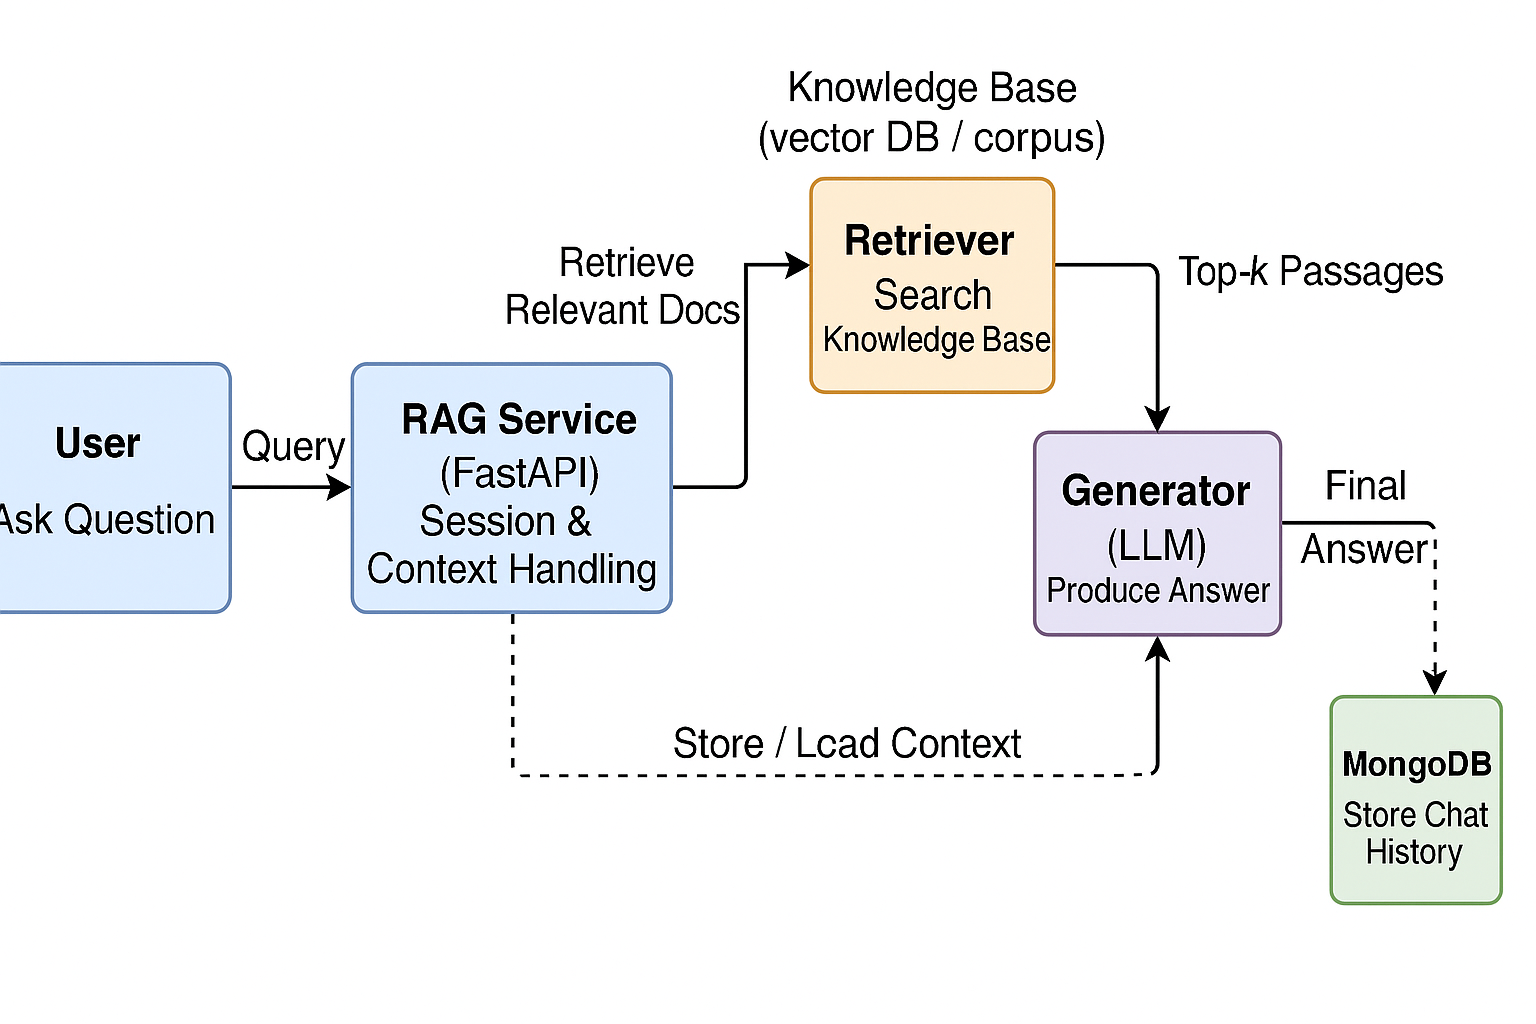
\includegraphics[width=0.75\linewidth]{images/AI_system_design.png}
%     \caption{Chat Task Workflow}
%     \label{fig:placeholder}
% \end{figure}

\textbf{RagFlow} is an external service handling document retrieval, reranking, and context-grounded generation and it exposes /api/v1/chats and OpenAI-compatible completion endpoints. Ragflow is easily deployed by \textbf{docker} and easy to use. All the chatting sessions are stored in MongoDB. It stores chat sessions, message history, and timestamps which makes Multi-round conversation available. It also supports querying, session resumption, and lightweight analytics.

% \section{Combined Investment Recommendation Module}

% This module will form a core part of our application. It will function as a semi-automated/AI-augmented Financial Research analyst (FRA). A FRA is a sector-specific or stock-specific expert who goes deep into their area/stock of expertise and tries to analyse how the sector or company will perform in the short-term and mid-term future. Their reports help investors make decisions.

% The main aim of our “Combined Investment Recommendation Module”, hereafter “CIRM” is to give all its research on any stock or any sector based on publicly available data like company reports, past experience, and domain knowledge, news, etc. We will then compare it with other analysts’ predictions to see how it has performed and to improve it. The module should also be able to revise its prediction based on news. “Combined” refers to quantitative + qualitative, multiple data sources, etc.

% In brief, Its purpose is to analyze stocks or sectors listed on Indian exchanges (NSE / BSE), aggregate data sources, run quantitative and qualitative analysis, and produce strategic reports and investment‐recommendations (risk/return / scenarios) that are transparent, defensible, and updatable.

% Our goal will be enabling an LLM in performing sentiment analysis and extracting signals from unstructured data like earnings calls, market news, and corporate filings.
% This section explains how the CIRM will be structured (conceptually), the modules, workflows, and how things connect, in a high-level way without overpromising.

% \begin{enumerate}
% 	\item Module architecture
%             \begin{itemize}
%                 \item[·] Analytics & Metrics Module: compute quantitative metrics, risk metrics, scenario modelling.
%                 \item[·] Qualitative / Text Analysis Module: process news, disclosures, risks, sentiment; extract risk factors, regulatory events.
%                 \item[·] Decision / Recommendation Module: integrates quantitative & qualitative insights, produces structured output.
%                 \item[·] Reporting & Visualization Module: generate reports with data, charts, assumptions, confidence levels.
%             \end{itemize}
% 	\item Workflow
%             \begin{itemize}
%                 \item[·] Regular update cycle (say, quarterly + event-driven): Pull in new filings, market data, sector / regulatory updates.
%                 \item[·] Triggered analyses when major events: earnings release, regulatory announcement, large price move, etc.
%                 \item[·] Peer benchmarking and scenario generation.
%             \end{itemize}
% 	\item User / Stakeholder Interface
%             \begin{itemize}
%                 \item[·] Analysts can view raw data, metrics, tweak assumptions).
%                 \item[·] Reports accessible by management / clients.
%             \end{itemize}
% 	\item Regulatory / Compliance Considerations (India / SEBI)
%             \begin{itemize}
%                 \item[·] Use only public / legally disclosed information.
%                 \item[·] Be cautious about forward-looking statements; label assumptions.
%                 \item[·] For PMS / advisory services ensure disclosures of risk, past returns, disclaimers.
%                 \item[·] Data privacy / corporate governance must be respected.
%             \end{itemize}
% \end{enumerate}














